%& --translate-file=cp1250pl.tcx
\documentclass[10pt,a4paper]{book}
\usepackage{polski}
\usepackage{amsmath}
\usepackage{amsfonts}
\usepackage{amssymb}
\usepackage{graphicx}
\usepackage{verbatim}
\usepackage{hyperref}
\usepackage{todonotes}
\author{Jakub Mozaryn, Jan Klimaszewski}
\title{Sterowanie Mechanizm�w Wielocz�onowych}
\begin{document}
	\maketitle
	\tableofcontents
	
	%ROZDZIA�Y
	
%ROZDZIA� 1
\chapter{Opis mechanizm�w wielocz�onowych - Janek+Kuba}
  W rozdziale przedstawiono podstawy matematyczne i fizyczne s�u��ce do opisu
  robot�w o wielu stopniach swobody (mechniazm�w wielocz�onowych). Przedstawiono model robota w przestrzeni zmiennych stanu. Opisano spos�b symulacji komputerowej dynamiki robota.	
  \section{Model geometrii, kinematyki i dynamiki mechanizm�w wielocz�onowych.}

  \subsection{Model geometrii - Janek}
  W pracy rozwa�any jest robot o pojedynczym �a�cuchu kinematycznym, sk�adaj�cy
  si� z cz�on�w po��czonych przegubami. Ka�dy z przegub�w posiada jeden stopie� swobody. W dalszej cz�ci pracy rozwa�any b�dzie robot o $n$-stopniach swobody z przegubami typu obrotowego, gdy� tylko przeguby tego typu wyst�puj� w rozwa�anym w pracy robocie PUMA 560. Przyj�to, �e dla robota o $n$-przegubach ponumerowanych od 1 do $n$ istnieje $n$+1 cz�on�w ponumerowanych od 0 do $n$. Cz�on o numerze 0 nazywany jest cz�onem bazowym, natomiast cz�on $n$ jest cz�onem z elementem wykonawczym. Przegub i ��czy cz�ony o numerach $i$-1 i $i$. Z ka�dym z cz�on�w zwi�zany jest uk�ad wsp�rz�dnych o tym samym numerze.
  %
  \subsection{Model kinematyki - Janek}
  Dla okre�lenia uk�ad�w wsp�rz�dnych kartezja�skich, kt�re b�d� przyporz�dkowane
  w odpowiedni spos�b do cz�on�w i przegub�w przyj�to notacj� Denavita-Hartenberga
  \cite{hartenberg:1955}, kt�rej podstawy zamieszczono na Rys. \ref{fig:1}:

  \begin{figure}[htb!]
	  \begin{center}
		  \includegraphics[width=1\linewidth]{figures/fig1}
		  %\\[1em]%
		  \caption{Standardowa notacja Denavita � Hartenberga (przyk�ad dw�ch obrotowych przegub�w $i$-1 oraz $i$), $a_i$ - d�ugo�� cz�onu, odleg�o�� od osi $z_i-1$ do osi $z_i$ mierzona wzd�u� osi $x_i$, $\alpha_i$ � k�t skr�cenia, k�t mi�dzy osiami $z_i-1$ i $z_i$ mierzony wok� osi $x_i$, $d_i$ - odsuni�cie cz�on�w,
			  odleg�o�� od �rodka uk�adu $i-1$ do osi $x_i$ mierzona wzd�u� osi $z_i-1$, $\theta_i$ - k�t konfiguracji, k�t mi�dzy osiami $x_i-1$ i $x_i$ mierzony wok� osi $z_i-1$ } \label{fig:1}
	  \end{center}                                         
  \end{figure}

  Po okre�leniu parametr�w uk�ad�w wsp�rz�dnych kartezja�skich mo�na wyznaczy�
  jednorodne macierze przekszta�ce� okre�laj�cych orientacj� i po�o�enie uk�adu $i$ wzgl�dem uk�adu $i-1$ \cite{fu:1987}:

  \begin{equation}
  ^{i-1}T{i}=T_{z,\theta}T_{z,d}T_{x,a}T_{x,\alpha}
  \end{equation}\label{eq:1}
  %
  gdzie: $^{i-1}T{i}$ - jednorodna macierz przekszta�cenia uk�adu $i-1$ wzgl�dem uk�adu $i$,$T_{z,\theta}$ - jednorodna macierz obrotu uk�adu $i$ wzgl�dem uk�adu $i-1$ wok� osi $z_i-1$ o k�t $\theta_i$, $T_{z,d}$ - jednorodna macierz przesuni�cia uk�adu $i$ wzgl�dem uk�adu $i-1$ o $d_i$ wzd�u� osi $z_i-1$,$T_{x,a}$ -  jednorodna macierz przesuni�cia uk�adu $i$ wzgl�dem uk�adu $i-1$ o $a_i$ wzd�u� osi $x_i$. ,$T_{x,\alpha}$-jednorodna macierz obrotu uk�adu $i$ wzgl�dem uk�adu $i-1$ wok� osi $x_i$ o k�t $\alpha_i$. 

  Macierze te wyra�one s� nast�puj�cymi zale�no�ciami:
  %
  \begin{equation}
  T_{z,\theta}=\left[\begin{array}{cccc}
  \cos{\theta_i} & -\sin{\theta_i} & 0 & 0 \\ 
  \sin{\theta_i} & \cos{\theta_i} & 0 & 0 \\ 
  0 & 0 & 1 & 0 \\ 
  0 & 0 & 0 & 1
  \end{array}\right] 
  \end{equation}\label{eq:2}
  %
  \begin{equation}
  T_{z,d}=\left[\begin{array}{cccc}
  1 & 0 & 0 & 0 \\ 
  0 & 1 & 0 & 0 \\ 
  0 & 0 & 1 & d_{i} \\ 
  0 & 0 & 0 & 1
  \end{array}\right] 
  \end{equation}\label{eq:3}
  %
  \begin{equation}
  T_{x,a}=\left[\begin{array}{cccc}
  1 & 0 & 0 & a_{i} \\ 
  0 & 1 & 0 & 0 \\ 
  0 & 0 & 1 & 0 \\ 
  0 & 0 & 0 & 1
  \end{array}\right] 
  \end{equation}\label{eq:4}
  %
  \begin{equation}
  T_{x,\alpha}=\left[\begin{array}{cccc}
  1 & 0 & 0 & 0 \\ 
  0 & \cos{\alpha_i} & -\sin{\alpha_i} & 0 \\ 
  0 & \sin{\alpha_i} & \cos{\alpha_i} & 0 \\ 
  0 & 0 & 0 & 1
  \end{array}\right] 
  \end{equation}\label{eq:5}
  %
  Wykorzystuj�c jednorodne macierze przekszta�ce� mo�na obliczy� wsp�rz�dne
  punktu w $m$-tym uk�adzie, znaj�c wsp�rz�dne tego samego punktu w $k$-tym uk�adzie
  (zak�adaj�c, �e $k>m$), jest to tzw. proste zadanie kinematyki. Zale�no�� t� wyznacza si�
  korzystaj�c z wyra�enia \cite{fu:1987}:
  %
  \begin{equation}
  P_{Am}=^{m}T_{k}P_{Ak}, k>m
  \end{equation}\label{eq:6}
  %
  gdzie:
  %
  \begin{equation}
  ^{m}T_{k}=^{m}T_{m+1}\quad ^{m+1}T_{m+2} \dots ^{k-1}T_{k}
  \end{equation}\label{eq:7}
  %
  $P_{Ak}=\left[\begin{array}{c}
  x_{Ak}\\ 
  y_{Ak}\\ 
  z_{Ak}\\ 
  1
  \end{array}\right]$ - jednorodny wektor wsp�rz�dnych punktu $A$ w $k$-tym uk�adzie wsp�rz�dnych

  $P_{Am}=\left[\begin{array}{c}
  x_{Am}\\ 
  y_{Am}\\ 
  z_{Am}\\ 
  1
  \end{array}\right]$ - jednorodny wektor wsp�rz�dnych punktu $A$ w $m$-tym uk�adzie wsp�rz�dnych
  %
  
  \subsection{Model dynamiki - Kuba}
  %
  Zale�no�ci opisuj�ce dynamik� robota o $n$-stopniach swobody mo�na wyznaczy�
  wykorzystuj�c uog�lnione r�wnanie Lagrange�a - Eulera o postaci \cite{fu:1987}
  %
  \begin{equation}
  \tau_{i}=\dfrac{d}{dt}\left(\dfrac{\delta L}{\delta \dot{q_{i}}}\right)-\dfrac{\delta L}{\delta q_{i}}, i=1,2,\dots,n
  \end{equation}\label{eq:8}
  gdzie: 
  $L$ - funkcja Lagrange�a (lagrangian) � funkcja potencja�u kinetycznego.
  %
  \begin{equation}
  L = K-P
  \end{equation}\label{eq:9}
  %
  $K$ - ca�kowita energia kinetyczna uk�adu, 
  $P$ - ca�kowita energia potencjalna uk�adu,
  $q_i$ - uog�lnione wsp�rz�dne uk�adu w przegubie $i$, $\tau_i$ - uog�lnione wymuszenia (si�y lub momenty) dzia�aj�ce w przegubie $i$
  \footnote{W robocie o przegubach obrotowych, jako uog�lnione wsp�rz�dne przyjmuje si�
  po�o�enia k�towe w przegubach, natomiast jako uog�lnione wymuszenia przyjmuje si�
  momenty nap�dowe w przegubach.}.

  Korzystaj�c z r�wna� Lagrange�a-Eulera, zale�no�ci opisuj�ce dynamik� robota z
  wszystkimi przegubami obrotowymi, mo�na przedstawi� w nast�puj�cy spos�b \cite{fu:1987}.
	  %
  \begin{equation}
  \tau=M(\theta)\ddot{\theta}+V(\theta, \dot{\theta})+G(\theta)
  \end{equation}\label{eq:10}
  %
  gdzie: $\tau\in R^{n}$ - wektor moment�w nap�dowych w przegubach, $n$ - ilo�� stopni swobody robota, 
  $M(\theta)\in R^{n\times n}$ - macierz bezw�adno�ci robota.
  $V(\theta, \dot{\theta})$ - wektor wyraz�w zawieraj�cych sk�adowe momentu zale�ne od si�
  od�rodkowych i Coriolisa, $G(\theta)\in R^{n}$- wektor wyraz�w zawieraj�cych sk�adowe momentu zale�ne od si�
  grawitacji, $\theta\in R^{n}$ - wektor po�o�e� k�towych w poszczeg�lnych przegubach.

  \textbf{Macierz $M(\theta)\in R^{n\times n}$}

  Elementy macierzy bezw�adno�ci wyznacza si� korzystaj�c z zale�no�ci:

  \begin{equation}
  m_{ik}=\sum_{j=\max(i,k)}^{n}Tr(U_{jk}J_{j}U_{jk}^{T}), i,k=1,2,\dots,n
  \end{equation}\label{eq:11}
  gdzie:
  \begin{equation}
  U_{jk}\equiv \dfrac{\delta ^{0}T_{i}}{\delta \theta_{j}}=
  \left\{\begin{array}{l}
  ^{0}T_{j-1}Q ^{j-1}T_{i}, \text{dla} j\leq i\\ 
  0, \text{dla} j>i
  \end{array}\right. 
  \end{equation}\label{eq:12}
  %
  \begin{equation}
  Q=\left[ \begin{array}{cccc}
  0 & -1  & 0 & 0 \\ 
  1 & 0 & 0 & 0 \\ 
  0 & 0 & 0 & 0 \\ 
  0 & 0 & 0 & 0
  \end{array} \right] \text{- dla przegubu obrotowego}
  \end{equation}\label{eq:13}
  %
  $J_{i}$ - jednorodna macierz inercji cz�onu $i$ wyra�ona zale�no�ci�:
  %
  \begin{equation}
  \begin{array}{l}
  J_{i}=\int r_{i}r_{i}^{T}dm=\\
  \left[ \begin{array}{cccc}
  \dfrac{-I_{XXi}+I_{YYi}+I_{ZZi}}{2} & I_{XYi} & I_{XZi} & m_{i}\overline{x}_{i} \\ 
  I_{XYi} & \dfrac{I_{XXi}-I_{YYi}+I_{ZZi}}{2} & I_{YZi} & m_{i}\overline{y}_{i} \\ 
  I_{XZi} & I_{YZi} & \dfrac{I_{XXi}+I_{YYi}-I_{ZZi}}{2} & m_{i}\overline{z}_{i} \\ 
  m_{i}\overline{x}_{i} & m_{i}\overline{y}_{i} & m_{i}\overline{z}_{i} & m_{i}
  \end{array} \right] 
  \end{array}
  \end{equation}\label{eq:14}
  %
  $I_{XXi}$,$I_{YYi}$,$I_{ZZi}$ - masowe momenty bezw�adno�ci cz�onu $i$, $I_{XYi}$,$I_{XZi}$,$I_{YZi}$ - masowe momenty dewiacji cz�onu $i$, $r_{i}=[x_{i}\quad y_{i} ]\quad z_{i}]^{T}$ - jednorodny wektor wsp�rz�dnych �rodka masy cz�onu $i$ wyra�ony w
  $i$-tym uk�adzie wsp�rz�dnych, $Tr(A)=\sum_{i=1}^{n}a_{ii}$ - �lad macierzy kwadratowej $A\in R^{n\times n}$.

  \textbf{Wektor $V(\theta, \dot{\theta})$ ma posta�}

  \begin{equation}
  V(\theta, \dot{\theta})=[V_{1},V_{2},\dots,V_{n}]^{T}
  \end{equation}\label{eq:15}

  Elementy wektora $V(\theta, \dot{\theta})$ mo�na wyznaczy� korzystaj�c z nast�puj�cych zale�no�ci:

  \begin{equation}
  V_{i}=\dot{\theta}^{T}H_{i}\dot{\theta}
  \end{equation}\label{eq:16}

  \begin{equation}
  H_{i}\in R^{n\times n}, i=1,2,\dots,n
  \end{equation}\label{eq:17}

  \begin{equation}
  h_{ikl}=\sum_{j=\max(i,k,l)}^{n}Tr(U_{jkl}J_{j}U_{ji}^{T}), i,k,l=1,2,\dots,n
  \end{equation}\label{eq:18}

  gdzie:
  \begin{equation}
  U_{ijk}\equiv \dfrac{\delta ^{0}U_{ij}}{\delta \theta_{k}}=
  \left\{\begin{array}{l}
  ^{0}T_{j-1}Q_{j} ^{j-1}T_{k-1} Q_{k} ^{k-1}T_{i}, \text{dla} j\leq k\leq i\\ 
  ^{0}T_{k-1}Q_{k} ^{k-1}T_{j-1} Q_{j} ^{j-1}T_{i}, \text{dla } k\leq j\leq i\\ 
  0, \text{dla } j>i \text{ lub } i<k
  \end{array}\right. 
  \end{equation}\label{eq:19}
  %
  \textbf{Wektor $G(\theta)$ ma posta�}

  Elementy wektora $G(\theta)$ mo�na wyznaczy� korzystaj�c z zale�no�ci:

  \begin{equation}
  g_{i}=\sum_{j=i}^{n}(-m_{j}\overline{g}U_{ij} ^{j}\overline{r}_{j}), i=1,2,\dots,n
  \end{equation}\label{eq:20}

  gdzie: $\overline{g}=[g_{x}\quad g_{y}\quad g_{x}\quad 0]^{T}$ -jednorodny wektor grawitacji wyra�ony w bazowym uk�adzie
  wsp�rz�dnych, $\sqrt{\overline{g}\overline{g}^{T}}=9.8062 [m/s{2}]$ - na powierzcni ziemi, $m_{i}$ masa cz�onu $i$.

  Nale�y doda�, �e istnieje szereg innych metod wyznaczania r�wna� dynamiki robota,
  np. metoda Newtona-Eulera, uog�lniona metoda d�Alamberta \cite{fu:1987},
  metoda Christoffela-Lagrange�a, metoda Walkera-Orina \cite{hejmo:1997}. Ich powstanie
  wynik�o g��wnie z potrzeby stworzenia szybkich algorytm�w do oblicze� numerycznych.
  Dok�adniejsz� analiz� i por�wnanie algorytm�w mo�na znale�� w \cite{fu:1987,hejmo:1997}.
  W dalszej cz�ci pracy wykorzystywany jest algorytm Lagrange�a-Eulera.
  Wyznaczona tym sposobem posta� r�wna� dynamiki \ref{eq:10} pozwala na �atw� analiz� w�a�ciwo�ci robota, zaprojektowania uniwersalnego algorytmu do jego symulacji, oraz
  syntez� uk�adu sterowania.
  %
  \subsection{W�a�ciwo�ci strukturalne modelu dynamiki}
  %
  \par Model matematyczny robota (\ref{eq:10}) posiada charakterystyczne w�asno�ci strukturalne. S� one cz�sto wykorzystywane podczas weryfikacji poprawno�ci modeli otrzymanych r�nymi metodami w trakcie projektowania i analizy uk�ad�w sterowania robot�w. Podstawowe w�asno�ci, kt�re b�d� wykorzystywane w pracy, s� nast�puj�ce \cite{tourassis:properties,swider:phd,morecki:podstawy,lewis:neuralcontrol}
  %
  
  \par \textbf{W�asno�ci strukturalne modelu robota ({WMR})}
  %
  \begin{description}
  	%
  	\item[WMR.1] Macierz inercji $M(q)$ jest symetryczna
  	%
  	\begin{equation}\label{2.4.1}%{2.17}
  	M(q)=M^{T}(q)
  	\end{equation}
  	%
  	\item[WMR.2] Macierz inercji $M(q)$ jest dodatnio okre�lona
  	%
  	\begin{equation}\label{2.4.2}%{2.18}
  	x^{T}M(q)x > 0 \qquad \forall x=[x_{i}]_{n \times 1}, x \neq 0
  	\end{equation}
  	%
  	\item[WMR.3] Elementy $m_{i,j}(q)$ macierzy inercji $M(q)$ nie zale�� od przemieszcze� uog�lnionych w 'aktualnym' przegubie i przegubach 'poprzednich'
  	%
  	\begin{equation}\label{2.4.4}%{2.20}
  	m_{i,j}(q)=m_{i,j}(q_{k+1},q_{k+2}, \ldots, q_{n}), \ \mathrm{gdzie} \ k=\min(i,j), \ \forall i,j=1,\ldots,n
  	\end{equation}
  	%
  \end{description}
  %
  Z w�asno�ci \emph{WMR.1} - \emph{WMR.3} wynikaj� nast�puj�ce wnioski
  %
  \begin{enumerate}
  	%
  	\item Macierz $M(q)$ jest nieosobliwa
  	%
  	\begin{equation}\label{2.4.3}
  	\text{det}[M(q)]\neq 0
  	\end{equation}
  	%
  	\item Mo�na dokona� dekompozycji macierzy $M(q)$
  	%
  	\begin{equation}\label{2.4.3a}
  	M(q)=P^{T}P \qquad \det{P}\neq 0
  	\end{equation}
  	%
  	\item �aden element macierzy inercji nie zale�y od przemieszczenia uog�lnionego w pierwszym przegubie, natomiast element $m_{n,n}$ nie zale�y od przemieszcze� uog�lnionych w �adnym z przegub�w i ma warto�� sta��.
  	%
  	\item Odwr�cona macierz inercji $\bar{M}(q)=[\bar{m}_{i,j}(q)]_{n \times n}$ jest symetryczna
  	%
  	\begin{equation}\label{2.6.9}%{2.17}
  	\bar{M}(q)=M(q)^{-1}=\bar{M}^{T}(q)
  	\end{equation}
  	%
  	\item Odwr�cona macierz inercji $\bar{M}(q)$ jest dodatnio okre�lona
  	%
  	\begin{equation}\label{2.6.10}%{2.18}
  	x^{T}\bar{M}(q)x > 0 \qquad \forall x=[x_{i}]_{n \times 1}, x \neq 0
  	\end{equation}
  	%
  	\item Ka�dy element odwr�conej macierzy inercji $\bar{M}(q)$ jest funkcj� przemieszcze� uog�lnionych we wszystkich przegubach opr�cz pierwszego
  	%
  	\begin{equation}\label{2.6.12}%{2.20}
  	\bar{m}_{i,j}(q)=\bar{m}_{i,j}(q_{2}, \ldots, q_{n}) \qquad \forall i,j=1,\ldots,n
  	\end{equation}
  	%
  \end{enumerate}
  %
  \par Model matematyczny robota o $n$-stopniach swobody z czasem dyskretnym mo�na otrzyma� aproksymuj�c pochodne przemieszcze� uog�lnionych \cite*{kurek:neural} (r�niczkowanie metod� \emph{Eulera})
  %
  \begin{equation}\label{3.1.1}
  \dot{q}(k)\approx\frac{q(k)-q(k-1)}{T_{p}}
  \end{equation}
  %
  \begin{equation}\label{3.1.2}
  \ddot{q}(k)\approx\frac{\dot{q}(k+1)-\dot{q}(k)}{T_{p}}\approx\frac{q(k+1)-2q(k)+q(k-1)}{{T_{p}}^2}
  \end{equation}
  %
  gdzie $T_{p}$ - okres pr�bkowania, $k$ - czas dyskretny, $t=kT_{p}$.
  %
  \par Po podstawieniu zale�no�ci (\ref{3.1.1}) i (\ref{3.1.2}) do r�wnania (\ref{eq:10}) otrzymuje si� model z czasem dyskretnym robota w postaci r�wna� \emph{Lagrange'a - Eulera}
  %
  \begin{equation}\label{3.1.3}
  M[q(k)]\frac{q(k+1)-2q(k)+q(k-1)}{{T_{p}}^2}+V[q(k),q(k-1)]+G[q(k)]=\tau(k)
  \end{equation}
  %
  gdzie, analogicznie jak w modelu (\ref{eq:10}), $M[q(k)]=[m_{i,j}[q(k)]]_{n \times n}$ - macierz inercji (bezw�adno�ci) robota, $V[q(k),q(k-1)]=[v_{i}[q(k),q(k-1)]]_{n \times 1}$ - wektor oddzia�ywa� zale�nych od si� od�rodkowych i si� \emph{Coriolisa}, $G[q(k)]=[g_{i}[q(k)]]_{n \times 1}$ - wektor oddzia�ywa� zale�nych od si� grawitacji.
  %
  \par Model z czasem dyskretnym robota (\ref{3.1.3}) zachowuje w�asno�ci strukturalne modelu robota \emph{WMR.1} - \emph{WMR.3}.
  %
  \section{Opis mechanizm�w wielocz�onowych w przestrzeni stanu.}
  %
  R�wnanie dynamiki robota w przestrzeni zmiennych stanu mo�na wyznaczy� w  oparciu o macierzowe r�wnanie dynamiki (\ref{eq:10}). Definiuj�c wektor stanu dla robota w  postaci \cite{fu:1987}:
 %
 \begin{equation}
 x=\left[\begin{array}{c}
 x_{1}\\ 
 x_{2}
 \end{array}  \right]=\left[\begin{array}{c}
 \theta \\ 
 \dot{\theta}
 \end{array}  \right]
 \end{equation}
  %
  oraz przyjmuj�c, �e wej�ciami do uk�adu s� sygna�y steruj�ce $\tau$ , natomiast wyj�ciami
  po�o�enia k�towe $\theta$ , r�wnanie dynamiki (\ref{eq:10}) mo�na wyrazi� w przestrzeni zmiennych
  stanu jako
  %
   \begin{equation}\label{eq:21}
  \begin{array}{l}
  \dot{x}=\left[\begin{array}{c}
  x_{2}\\ 
  -M^{-1}(\theta)[V(\theta, \dot{\theta})+G(\theta)]
  \end{array}  \right]+\left[\begin{array}{c}
  0 \\ 
  M^{-1}(\theta)
  \end{array}  \right]\tau
  \\
  y=\left[I \quad 0 \right]x
  \end{array}
  \end{equation}
  %
  Stosuj�c standardowe oznaczenia modeli stanu, uk�ad r�wa� (\ref{eq:21}) zapisuje si� nast�puj�co
  %
  \begin{equation}\label{eq:22}
  \begin{array}{l}
  \dot{x}=A(x)+B(x)\tau
  \\
  y=Cx
  \end{array}
  \end{equation}
  gdzie:
  \begin{equation}\label{eq:23}
  A(x)=\left[\begin{array}{c}
  x_{2}\\ 
  -M^{-1}(\theta)[V(\theta, \dot{\theta})+G(\theta)]
  \end{array}  \right]
  \end{equation}
  %
  \begin{equation}\label{eq:24}
  B(x)=\left[\begin{array}{c}
  0 \\ 
  M^{-1}(\theta)
  \end{array}  \right]
  \end{equation}
  %
   \begin{equation}\label{eq:24}
  C(x)=\left[I \quad 0 \right]
  \end{equation}
  %
  Charakterystycznymi w�a�ciwo�ciami robota jako obiektu sterowania s� nieliniowo�ci
  wynikaj�ce z istnienia si� Coriolisa i si� od�rodkowych, zmienno�� parametr�w uk�adu w
  czasie, oraz sprz�enia pomi�dzy wszystkimi stopniami swobody.
  \section{Identyfikacja parametr�w kinematycznych i dynamicznych robot�w.
  }
  \section{Zastosowanie kwaternion�w.}
  
  \section{Otwarte i zamkni�te �a�cuchy kinematyczne.}
  
  \section{Uk�ady niedosterowane.}
  %
  Uk�ady niedosterowane (ang. \textit{underactuated systems}) nale�� do szerokiej klasy urz�dze� i system�w wyst�puj�cych w robotyce oraz teorii sterowania. W og�lno�ci przez \textbf{uk�ady niedosterowane} rozumie si� systemy, w kt�rych liczba mo�liwych wymusze� (wej�� uk�adu) jest mniejsza od liczby stopni swobody (wyj�� uk�adu). W przypadku uk�ad�w sterowania, omawiane zagadnienie sprowadza si� do proces�w, w kt�rych liczba sterowanych wyj�� jest mniejsza od liczby dost�pnych sygna��w steruj�cych. 
  
  Uk�ady niedosterowane w teorii sterowania s� interesuj�ce ze wzgl�du na swoje w�asno�ci. Niedob�r element�w wykonawczych powoduje, �e generowane sterowania dzia�aj� jednocze�nie na kilka wyj�� i nie ma mo�liwo�ci na niezale�ne wp�ywanie na ka�de z nich. 
  
  W efekcie algorytm regulacji kontroluj�cy takie urz�dzenie musi uwzgl�dnia� wiele wymaga� naraz i wybiera� rozwi�zanie dla zadanej sytuacji. 
  Badania takich uk�ad�w by�y prowadzone mi�dzy innymi w zakresie wykorzystania teorii chaosu do sterowania niedosterowanym systemem satelit�w \cite{pang:2015}, sterowania �lizgowego nieliniowymi uk�adami niedosterowanymi \cite{khan:2015} lub u�ycia adaptacyjnego modelu z predykcj� 
  do sterowania robotem i minimalizacji zu�ycia energii \cite{ahmad:2016}.
  Jednym z najprostszych urz�dze� niedosterowanych jest wahad�o odwr�cone. Konstrukcja wahad�a pozwala na niezale�ny ruch wzd�u� osi prowadnicy, na kt�rej jest zamontowane oraz obr�t wok� w�asnej osi. Pomimo prostej konstrukcji wahad�o odwr�cone jest uk�adem cz�sto wykorzystywanym w celu testowania r�nego rodzaju algorytm�w regulacji. 
  
  Ze wzgl�du na swoj� budow�, wahad�o posiada chwiejny punkt r�wnowagi w pozycji pionowej, kt�rego opuszczenie powoduje utrat� stabilno�ci i upadek do stabilnej pozycji dolnej. Pomimo prostego opisu matematycznego jego zachowa�, jest to obiekt nieliniowy, dla kt�rego realizacja sterowania nie jest prosta.
  %
  \section{Uk�ady nieholonomiczne.}
  \section{Kolizje.}
  %-----

	
%Rodzia� 2
\newpage
\chapter{Standardowe modele uk�ad�w wielocz�onowych}
  \section{wahad�o odwr�cone}
  \section{acrobot}
  \section{maszyny krocz�ce}
%-----

	
%Rodzia� 3
\newpage
\chapter{Planowanie trajektorii ruchu robota}
  \section{Planowanie trajektorii ruchu robota w przestrzeni wewn�trznej, zewn�trznej i kartezja�skiej}
  \section{Koordynacja ruchu robot�w w przestrzeni zada�}
  \section{Planowanie ruchu jako przeszukiwanie}
%-----

	
%Rodzia� 4
\newpage
\chapter{Sterowanie w przestrzeni przegub�w - Kuba}
  \section{Serwomechanizmy przegub�w}
  \section{Sterowanie w przestrzeni przegub�w}
  
  \subsection{Metoda odwrotnego modelu}
  Jedn? z najbardziej popularnych metod sterowania pozycyjnego w robotyce jest metoda odwrotnego modelu. Metoda modelu odwrotnego jest stosowan? w robotyce metod? linearyzacji i dekompozycji modelu matematycznego manipulatora, dzi?ki kt�rej mo?na sterowa? niezale?nie wszystkimi ramionami robota z wykorzystaniem technik sterowania obiektami liniowymi. Metoda odwrotnego modelu ma t? zalet? w por�wnaniu z innymi metodami linearyzacji (np. rozwini?cie w szereg Taylora) modelu, ?e kompensuje nieliniowo?ci w ca?ym zakresie zmian wsp�?rz?dnych z??czowych, a nie tylko w pobli?u punktu, wok�? kt�rego linearyzujemy model. 
    
  Na rys. \ref{rys:4_1} przedstawiony jest og�lny schemat sterowania robota (mechanizmu wielocz?onowego) z wykorzystanim modelu odwrotnego.
  %
    \begin{figure}[htb!]
  	\begin{center}
  		\includegraphics[width=1\linewidth]{figures/fig4_1}
  		\caption{Schemat sterowania robota z wykorzystaniem modelu odwrotnego}\label{rys:4.1}
  	\end{center}
  \end{figure}

W strukturze sterowania mo?emy wyr�?ni? dwie p?tle sprz??enia zwrotnego:
%
\begin{itemize}
\item	P?tl? wewn?trzn? linearyzuj?c? i rozdzielaj?ca prawo sterowania na cze?? modelow? oraz sprz??eniow?
\item	P?tl? zewn?trzn? sprz??enia zwrotnego pozwalaj?c? na sterowanie manipulatora w ??dany spos�b
\end{itemize}
%
Aby wyznaczy? odpowiednie sygna?y steruj?ce, nale?y wszystkie uk?ady zwi?zane z przegubami uniezale?ni? od siebie. Pozwoli to na uproszczenie problemu wyznaczenia sterowania do wyznaczenia sygna?�w steruj?cych dla sze?ciu odsprz?gni?tych uk?ad�w drugiego rz?du. Metody odsprz?gania przegub�w robota opisano m.in. w \cite{fu:1987}, \cite{craig:1995}.

Dany jest model robota opisany r�wnaniem \ref{eq:10}. Przyjmuj?c posta? wektora sygna?�w steruj?cych:
\begin{equation}
	\tau=P(x,t)\hat{\tau}+R(x,t),
\end{equation}\label{eq:4_1}
oraz przyjmuj?c, ?e:
\begin{equation}
P(x,t)=\hat{M}(x,t)
\end{equation}\label{eq:4_2}
%
\begin{equation}
R(x,t)=\hat{V}(x,t)+\hat{G}(x,t)
\end{equation}\label{eq:4_3}
%
mo?na rozdzieli? uk?ady zwi?zane z przegubami w r�wnaniu (\ref{eq:10}). Macierze $\hat{M}(x,t)$, $\hat{V}(x,t)$,$\hat{G}(x,t)$ s? oszacowaniami (estymatami) macierzy $M(x,t)$, $V(x,t)$,$G(x,t)$, w r�wnaniach Lagrange?a-Eulera, liczonymi wed?ug wzor�w podanych w rozdziale 1, na podstawie oszacowanych parametr�w robota. 

R�wnanie opisuj?ce dynamik? robota mo?na zapisa?, wykorzystuj?c
zale?no?ci (3.10) i (\ref{eq:4_1}), w postaci:
%
\begin{equation}
M(x,t)\ddot{q}+G(x)+V(x)=P(x,t)\hat{\tau}+R(x)
\end{equation}\label{eq:4_4}
%
Zak?adaj?c, ?e oszacowane parametry robota maj? te same warto?ci co parametry rzeczywiste,
r�wnanie (\ref{eq:4_4}) upraszcza si? do postaci:
%
\begin{equation}
M(x,t)\ddot{q}=\hat{M}(x,t)\hat{\tau}
\end{equation}\label{eq:4_5}
%
Zak?adaj?c, ?e macierz $M(x)$ jest macierz? nieosobliw?, oraz $M(x)= \hat{M}(x)$, w
wyniku odsprz?gni?cia uzyskuje si? sze?? niezale?nych uk?ad�w opisanych r�wnaniami drugiego rz?du, postaci:
%
\begin{equation}
\ddot{q}=\hat{\tau}
\end{equation}\label{eq:4_6}
%
Uk?ad (\ref{eq:4_6}) mo?na opisa? r�wnaniami w przestrzeni zmiennych stanu jako
%:
\begin{equation}
	\left\{\begin{array}{l}
	\dot{x_{i}}=Ax_{i}+B\hat{tau}\\
	y_{i}=Cx_{i}\\
	i=1,\dots,n
	\end{array}\right.
\end{equation}\label{eq:4_7}
gdzie
\begin{equation}
x_{i}=\left[\begin{array}{c}
q_{i}\\
\dot{q_{i}}
\end{array}\right],
A=\left[\begin{array}{cc}
0 & 1\\
0 & 0
\end{array}\right],
B=\left[\begin{array}{c}
0\\
1
\end{array}\right],
c=\left[1 \quad 0\right],
\end{equation}\label{eq:4_8}
%
G?�wnym wymaganiem przy stosowaniu metody odwrotnego modelu do sterowania jest konieczno?? zapewnienia dok?adnych oraz szybkich pomiar�w wsp�?rz?dnych z??czowych. Jest to silne za?o?enie, poniewa? pomiar parametr�w robota jest zawsze obarczony jest pewnym b??dem to nie wszystkie parametry modelu s? dok?adnie okre?lone. 
    \subsection{Transmitancja przegubu - Kuba}
    \subsection{Regulator po�o�enia przegubu - Kuba}
    \subsection{Regulator momentu przegubu - Janek}
    \subsection{Stabilno�� uk�adu regulacji i wska�niki jako�ci regulacji - Kuba}
  \section{Sterowanie adaptacyjne - Kuba}
%-----

	
%Rodzia� 5
\newpage
\chapter{Sterowanie w przestrzeni stanu - Kuba}
  \section{Regulator dla robota o wielu stopniach swobody}
  \section{Linearyzacja sprz�enia zwrotnego}
  \section{Dob�r funkcji Lapunova dla potrzeb sterowania mechanizm�w wielocz�onowych}
  \section{Sterownie pozycyjne i sterowanie nad��ne}
  \section{Projektowanie sterowania jako zadanie optymalizacji}
%-----

	
%Rodzia� 6
\newpage
\chapter{Sterowanie si�owe - Janek}
  \section{Sterowanie impedancyjne}
  \section{Sterowanie si�owe}
  \section{Sterowanie pozycyjno-si�owe}
  \section{Modele tarcia}
%-----

	
%Rodzia� 7
\newpage
\chapter{Sterowanie optymalne i sterowanie odporne}
  \section{Sterowanie o zmiennej strukturze mechanizm�w wielocz�onowych}
  \section{Sterowanie predykcyjne mechanizm�w wielocz�onowych}
  \section{Sterowanie LQR/LQG mechanizm�w wielocz�onowych}
%-----

	
%Rodzia� 8
\newpage
\chapter{Metody sztucznej inteligencji w sterowaniu mechanizm�w wielocz�onowych - Janek+Kuba}
  \section{Sieci neuronowe do modelowania mechanizm�w wielocz�onowych}
  \section{Regulator stanu mechanizmu wielocz�oowego oparty o sieci neuronowe}
  \section{Logika rozmyta w sterowaniu mechanizm�w wieloczlonowych}
  \section{Sterowanie ze wzmocnieniem mechanizm�w welocz�onowych}	


	%BIBLIOGRAFIA
	\bibliographystyle{unsrt}
	\bibliography{bib/bibliografia}
\end{document}}